%
% auth: Mattijs Korpershoek
% mail: <mattijs.korpershoek@gmail.com>
%

% {{{1 features
\section{Technical contributions}
\begin{FrameWithSubSection}
    \begin{itemize}
        \item Customer features
        \item Open-sourcing a core component
    \end{itemize}
\end{FrameWithSubSection}


% {{{1 Customer features
\subsection{Features for customers}
\begin{FrameWithSubSection}
    \begin{itemize}
        \item More than \emph{80} patches delivered
        \item Code used in Intel
    \end{itemize}
\end{FrameWithSubSection}

% {{{2 xml validation
\subsubsection{Xml Validation at build time}
\begin{frame}
    \frametitle{XML Validation at build time}
    % Decrire le nombre de fichiers erronés
\end{frame}

\begin{frame}
    \frametitle{XML Validation at build time}
    % montrer avant
\end{frame}

\begin{frame}
    \frametitle{XML Validation at build time}
    % montrer apres
\end{frame}

% {{{2 fixed point
\subsubsection{Fixed point parameter improvements}
\begin{frame}
    \frametitle{Fixed point parameter improvements}
    % probleme
\end{frame}

\begin{frame}
    \frametitle{Fixed point parameter improvements}
    % Illustration du problème
\end{frame}

% {{{1 Opensourcing
\subsection{Open-sourcing the Parameter-framework}
\begin{FrameWithSubSection}
    \begin{itemize}
        \item Core component of Intel Audio HAL
        \item Middleware standard
        \item Visibility
    \end{itemize}
\end{FrameWithSubSection}

\begin{FrameWithSubSection}
    \frametitle{Parameter-framework top contributors}
    \centering
    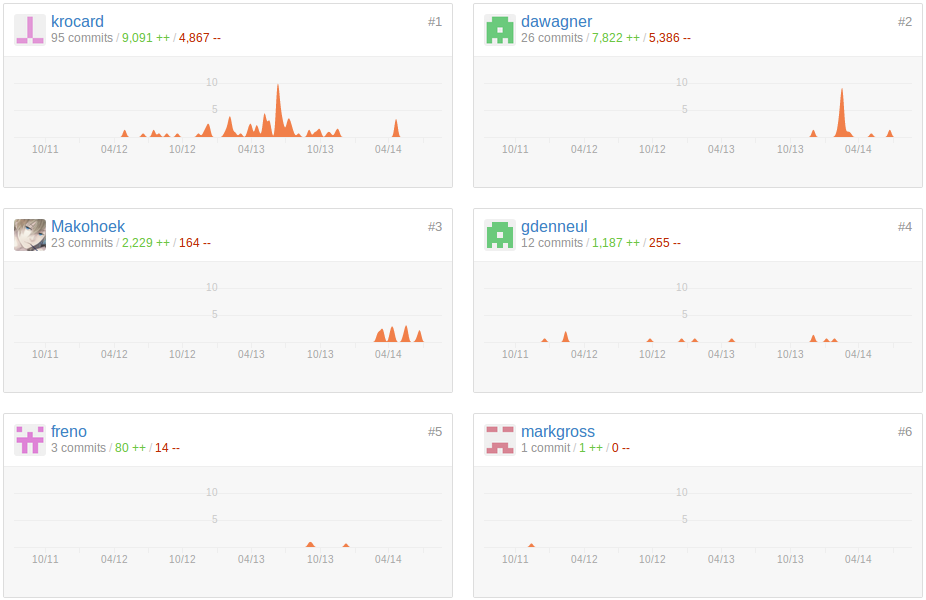
\includegraphics[width=\textwidth]{../../report/src/img/statsGitHub.png}
\end{FrameWithSubSection}


\begin{FrameWithSubSection}
    \frametitle{Newcomer documentation}
    \centering
    \begin{block}{Is component ready for open-sourcing?}
        \begin{itemize}
            \item Code review and study
            \item Documentation for external contributors
            \item More than 450 lines of documentation
        \end{itemize}
    \end{block}
\end{FrameWithSubSection}
